\chapter{Súvisiace práce}
\label{related-work}

V tejto kapitole uvádzam a v krátkosti popisujem existujúce práce, ktoré buď v minulosti vypracovávali vlastnú analýzu využívania NEL, alebo na tému NEL obsahujú dôležité poznatky.

\subsubsection{Vypracované analýzy}
\label{praca-veduceho}
\label{skript}

Existuje predošlá analýza zameraná na technológiu NEL, v ktorej sa pán Ing. Libor Polčák Ph.D. zameriava na získanie metrík ako celková využívanosť NEL a jeho konfigurácia.
Taktiež s jeho kolegom, Ing. Kamilom Jeřábkom, zistili, ktoré domény slúžia ako web servery určené pre uchovávanie zaslaných hlásení NEL.
V rámci tejto analýzy použili projekt HTTP Archive ako zdroj dát pre svoj prieskum.
Ako nástroj pre získavanie dát z uvedeného zdroja a ich ukladanie bol vyvinutý pomocný skript 
pánom Jeřábkom\footnote{\href{https://github.com/kjerabek/nel-http-archive-analysis}{https://github.com/kjerabek/nel-http-archive-analysis}}.
Časové obdobie, za ktoré bola analýza zhotovená, tvorili februárové mesiace každého roku od 2019 do 2023. 
Za toto obdobie sa podarilo zistiť, že počiatočné využitie NEL bolo 0\%, no vo februári roku 2023 stúplo na 11.73\% skúmaných domén.
Toto percento predstavuje z celkového zoznamu skúmaných domén približne 2,250,000 jedinečných domén.
Zistili tiež, že najviac domén využívaných ako web servery pre ukladanie zaslaných hlásení NEL vlastnila vo februári 2023 spoločnosť Cloudflare \cite{nel-http-archive}.

Ich prácu sem uvádzam z toho dôvodu, že okrem referencovania stavu pred vypracovaním mojej vlastnej analýzy tiež \textbf{používam nimi implementovaný skript} pre získavanie \mbox{a ukladanie} dát poskytovaných projektom HTTP Archive.

\begin{figure}[!htb]
\begin{center}
    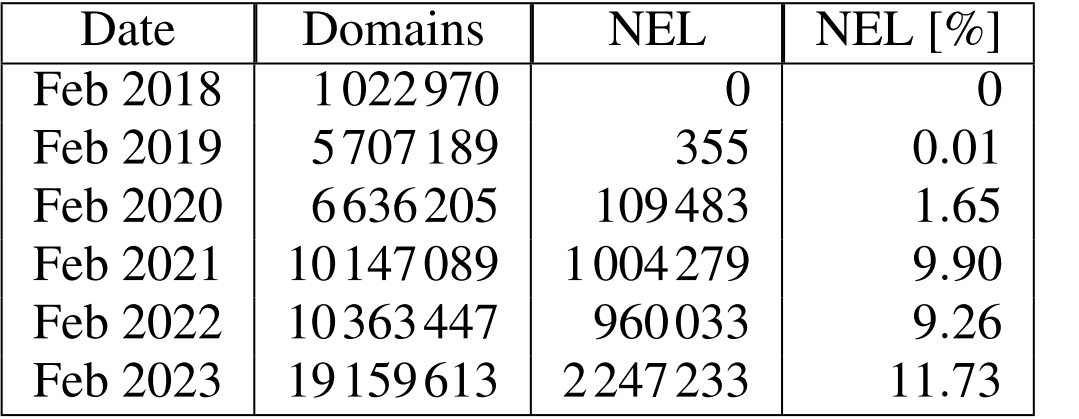
\includegraphics[width=0.5\linewidth]{obrazky-figures/polcak-analysis.png}
    \caption{\centering Hlavné výsledky analýzy vypracovanej vo vedeckom článku Ing. Libora Polčáka Ph.D. a Ing. Kamila Jeřábka. Obrázok je prebraný z ich práce.}
    \label{fig:polcak-analysis}
\end{center}
\end{figure}

\subsubsection{Dôležité poznatky}

Jedným z dôležitých zistení uvedených v existujúcich prácach je, že projekt HTTP Archive sa pri svojom prehľadávaní domén sústredí iba na zdroje referencované z domovskej stránky získanej pre danú doménu.
To znamená, že skúmajú iba malú čiastku zdrojov dostupných na cieľovej doméne a zvyšok jednoducho ignoruje.
Autori práce usúdili, že vzhľadom na tento fakt nie je možné vypracovať dostatočne presnú analýzu na základe dát poskytnutých iba projektom HTTP Archive \cite{nel-http-archive}.

Z toho dôvodu je nutné v mojej analýze navrhnúť aj iný spôsob skúmania stavu využitia technológie NEL.
To je zohľadnené v ďalšej kapitole, kde popisujem celkový návrh vypracovania svojej analýzy.
